\documentclass[]{article}
\usepackage{fullpage}
\usepackage{lastpage}
\usepackage[top=1in,bottom=1in,margin=1in]{geometry}
\usepackage{supertabular}
\usepackage{graphicx,tikz}	
%\usepackage{tkz-euclide}
%\usetkzobj{all}
\usetikzlibrary{calc}
\usepackage{array,multicol}
\usepackage{amsmath,amssymb}
\usepackage{enumitem}

\usepackage{fancyhdr}
\pagestyle{fancy}

\addtolength{\topmargin}{-0.25in}

\newcommand{\vect}[1]{\mathbf{#1}}
\DeclareMathOperator{\proj}{proj}

\fancypagestyle{plain}{
	\addtolength{\headheight}{0.485in}
	\rhead{\bf MATH 2574 (Calculus III) \\
		%\vspace{0.5pc}
		Fri 3 Feb 2017 \\}
	\rfoot{\footnotesize $\;$Quiz 2IC, p. \thepage\ (of \pageref{LastPage})
	}
\renewcommand{\headrulewidth}{0pt}
}
\fancyhf{}
\renewcommand{\headrulewidth}{0pt}
\rfoot{\footnotesize Quiz 2IC, p. \thepage\ (of \pageref{LastPage})$\;$}

\title{\vspace{-3.5pc} 
	\flushleft \bf \Large In-Class Quiz 2: \\ Functions of several variables (\S 12.1-12.2)}
\date{}

% % % % %
\begin{document}
\maketitle

\vspace{-3pc}
\noindent{\bf Directions:} This quiz is due at the end of lecture.  

\noindent\hrulefill

\begin{enumerate}

% % %
\item %{\bf 12.2 \#29} 
Match functions (a)-(d) with surfaces (A)-(D).
\begin{enumerate}
	\item $f(x,y)=\dfrac{6}{x-y}$
	\item $g(x,y)=\ln{(x^2+y^2)}$
	\item $h(x,y)=\dfrac{1}{1+x^2+y^2}$
	\item $p(x,y)=\cos{xy}$
\end{enumerate}
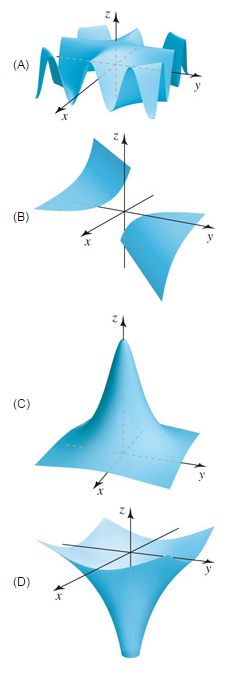
\includegraphics[scale=0.75]{Q2surfaces}

% % %
\item %{\bf 12.1 \#5}
To which coordinate axes are the following cylinders parallel in $\mathbb R^3$?
\begin{enumerate}
	\item $3z^2+2y^2=9$
	\item $x^2+y^2=9$
	\item $x^2+z^2=9$
\end{enumerate}	

% % % % %
\end{enumerate}
\end{document}